\documentclass[12pt]{article}

\usepackage{amsmath}
\usepackage{amssymb}
\usepackage{tikz}
\usetikzlibrary{matrix}


\newtheorem{lemma}{Lemma}
\newtheorem{theorem}{Theorem}
\newtheorem{remark}{Remark}

\def\a{\mathfrak{a}}
\def\Q{\mathbb{Q}}
\def\C{\mathbb{C}}
\def\OK{\mathcal{O}_K}
\def\Ok{\mathcal{O}_k}
\def\eps{\varepsilon}
\DeclareMathOperator{\Cl}{Cl}
%\def\errorexp{1-1/n}
\def\errorexp{1-\frac{2}{n+1}}

\title{An improved error term for counting $D_4$-quartic fields}
\author{Kevin J.~McGown \and Amanda Tucker}


\begin{document}

\maketitle

\begin{abstract}
We prove that the number of quartic fields $K$ with
discriminant $|\Delta_K|\leq X$ whose Galois closure is $D_4$  equals $CX+O(X^{5/8+\eps})$,
improving the error term in a well-known result of Cohen, Diaz y Diaz, and Olivier.
\end{abstract}


\section{Introduction}\label{S:intro}

Let $N_n(G,X)$ be the number of degree $n$ number fields with Galois closure $G$ and discriminant
$|\Delta_K|\leq X$.  It is an interesting problem to find asymptotic expressions for $N_n(G,X)$.
This is the subject of conjectures of Malle and Bhargava.
Among other things, this is connected to the inverse Galois problem and the Cohen--Lenstra heuristics for class groups.
See, for example, the papers~\cite{bhargava.mass, cohen.lenstra, malle1, malle2, kluners}.
We do not give a summary of the literature here.

In this investigation, we will focus on quartic fields whose Galois closure is $D_4$, the symmetry group of a square. 
Our main result is as follows:

\begin{theorem}\label{T:1}
We have
$$
N_4(D_4,X)=CX+O(X^{5/8+\eps})
$$
where
$$
  C=
  \frac{1}{2}
\sum_{\substack{[k:\Q]=2}}
\frac{1}{2^{r_2(k)}\Delta_k^2}
\frac{\zeta_k^*(1)}{\zeta_k(2)}
%\,,\qquad
%D=
%\frac{23}{640}
%\prod_{p}\left(1+\frac{3}{p}\right)\left(1-\frac{1}{p}\right)^3
\,.
$$
\end{theorem}
Here $\zeta_k(s)$ denotes the Dedekind zeta function of $k$ and $\zeta^*(1)$ denotes the
first non-vanishing Laurent coefficient of $\zeta(s)$ at $s=1$.  As is customary,
$r_1(k)$ and $2r_2(k)$ denote the number of real and complex embeddings, respectively. 

Previously, Cohen, Diaz y Diaz, and Olivier (see~\cite{cohen.diaz.olivier}) proved that
$N_4(D_4,X)=CX+O(X^{3/4+\eps})$.
In later numerical work (see~\cite{cohen.diaz.olivier2}), they suggest that it is ``reasonable to conjecture'' 
that the error is $O(X^{1/2+\eps})$, and that there may be a secondary term.
Theorem~\ref{T:1} strengthens the error term in their result.
Our proof follows their approach and appeals to some of the calculations in Section 3 of~\cite{cohen.diaz.olivier},
but we do not  make explicit use of the same Dirichlet series.
See Remark~\ref{R:1} in~\S\ref{S:proof} for additional comments on their conjecture in the context of our proof.

Late in the preparation of this manuscript we became aware that
Barquero-Sanchez, Masri, and Thorne
(see Theorem 2.4 of~\cite{barquero.masri.thorne})
already obtained an improvement to $O(X^{5/7 + \eps})$
for the closely related problem of counting $D_4$-quartic fields that
are totally imaginary extensions of totally real quadratic fields.

In the course of proving Theorem~\ref{T:1} we establish a result for counting relative
quadratic extensions for which the implicit constant in the error term only depends
on the degree of the base field.

\begin{theorem}\label{T:relative}
Let $k$ be a number field of degree $n\geq 2$.  We have
%$$
%\sum_{\substack{[K:k]=2\\N(\Delta_{K/k})\leq X}}1=
%\frac{1}{2^{r_2(k)}}
%\frac{\zeta_k^*(1)}{\zeta_k(2)}X
%+
%O_n\left(
%|\Cl^+(k)[2]|\cdot
%|\Delta_k|^{\frac{1}{n+1}}X^{\errorexp}(\log X)^{n-1}
%\right)
%\,.
%$$
\begin{align*}
&
\sum_{\substack{[K:k]=2\\N(\Delta_{K/k})\leq X}}1=
\frac{1}{2^{r_2(k)}}
\frac{\zeta_k^*(1)}{\zeta_k(2)}X
+
|\Cl^+(k)[2]|
\cdot
%\times
\\
&
\times
\begin{cases}
O\left(
%|\Cl^+(k)[2]|\cdot
|\Delta_k|^{1/3}\log|\Delta_k|\cdot X^{1/2}\log X
\right)
&
n=2
\\
O\left(
%|\Cl^+(k)[2]|\cdot
|\Delta_k|^{1/4}(\log|\Delta_k|)^2\cdot X^{1/2}(\log X)^3
\right)
&
n=3
\\
O_n\left(
%|\Cl^+(k)[2]|\cdot
|\Delta_k|^{\frac{1}{n+1}}X^{\errorexp}(\log X)^{n-1}
\right)
&
n>3
\end{cases}
\end{align*}
\end{theorem}
In the above, $\Cl^+(k)[2]$ denotes the $2$-torsion subgroup of the narrow class group of $k$.
%We emphasize that the implicit constant only depends on the degree $n$ of the extension.

We note in passing that other variations on the problem
of counting $D_4$-quartic fields have been investigated,
such as counting the fields when ordered by their Artin conductor, 
or over a general base field
(see~\cite{altug.ali.shankar.varma.wilson, BFSLV22}).
Our approach may yield improved error terms for these situations as well, although we have
not investigated this.

\section{Initial setup}
%In Cohen, Diaz y Diaz, and Olivier, the following equation appears (Corollary~2.2)
%$$
%\sum_{[k:\Q]=2}\sum_{[K:k]=2} 1
%=
%2\sum_{\substack{[K:\Q]=4\\G(K/\Q)=D_4}} 1
%+
%\sum_{\substack{[K:\Q]=4\\G(K/\Q)=C_4}} 1
%+
%3\sum_{\substack{[K:\Q]=4\\G(K/\Q)=V_4}} 1
%$$
The following is a truncated version of Corollary~2.2 of~\cite{cohen.diaz.olivier}:
\begin{equation}\label{E:fields}
\sum_{\substack{[k:\Q]=2\\
|\Delta_{k}|\leq \sqrt{X}}}
\;\;
\sum_{\substack{[K:k]=2\\N(\Delta_{K/k})\leq X/\Delta_k^2}}1
=
2\sum_{\substack{[K:\Q]=4\\G(K/\Q)=D_4\\|\Delta_{K}|\leq X}} 1
+
\sum_{\substack{[K:\Q]=4\\G(K/\Q)=C_4\\|\Delta_{K}|\leq X}} 1
+
3\sum_{\substack{[K:\Q]=4\\G(K/\Q)=V_4\\ |\Delta_{K}|\leq X}} 1
\,.
\end{equation}
In words, counting extensions that are quadratic over quadratic picks
up every $D_4$-quartic (up to isomorphism) exactly twice, every $V_4$-quartic 
exactly three times, and every $C_4$-quartic exactly once.  This is observed in
the following field diagram for the Galois closure $L$ of a generic $D_4$-quartic field $K_1$.
(Every line stands for a degree $2$ extension.)

\begin{center}
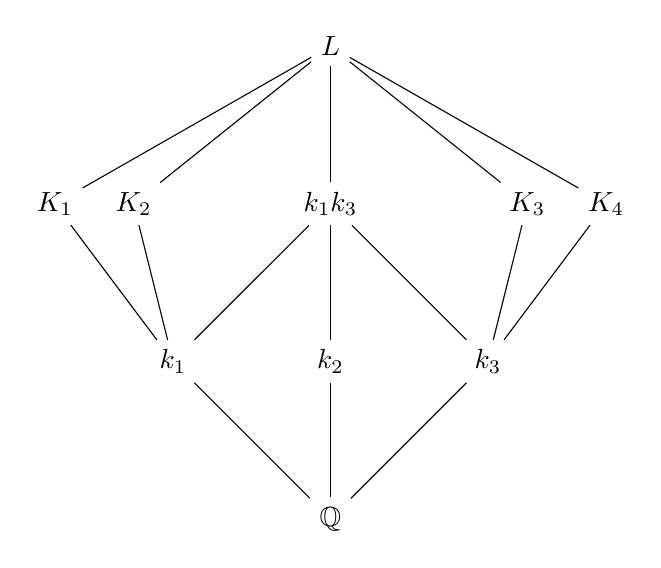
\begin{tikzpicture}
    \node (Q1) at (0,0) {$\Q$};
    \node (Q2) at (-2,2) {$k_1$};
    \node (Q3) at (0,2) {$k_2$};
    \node (Q4) at (2,2) {$k_3$};
    
    \node (Q5) at (-3.5,4) {$K_1$};
    \node (Q6) at (-2.5,4) {$K_2$};
    \node (Q7) at (0,4) {$k_1k_3$};
    \node (Q8) at (2.5,4) {$K_3$};
    \node (Q9) at (3.5,4) {$K_4$};
    \node (Q10) at (0,6) {$L$};




    \draw (Q1)--(Q2);
    \draw (Q1)--(Q3);
    \draw (Q1)--(Q4);
        
    \draw (Q2)--(Q5);
    \draw (Q2)--(Q6);

    \draw (Q2)--(Q7);
    \draw (Q3)--(Q7);
    \draw (Q4)--(Q7);

    \draw (Q4)--(Q8);
    \draw (Q4)--(Q9) ;

    \draw (Q5)--(Q10);
    \draw (Q6)--(Q10);

    \draw (Q8)--(Q10);
    \draw (Q9)--(Q10) ;

    \draw (Q7)--(Q10);

   
\end{tikzpicture}
\end{center}
The truncations in the subscripts in~(\ref{E:fields})
follow immediately from $\Delta_K=N(\Delta_{K/k})\Delta_k^2$, where $\Delta_{K/k}$ denotes the relative
discriminant.

The first term on the right of~(\ref{E:fields}) is what we want to count.
The next two terms on the right are $O(\sqrt{X})$ and $O(\sqrt{X}(\log X)^2)$,
respectively (see~\cite{baily}).
The main task is to deal with the innermost sum on the left, which counts relative
quadratic extensions.

\section{Counting relative quadratic extensions}

In this section, we consider the problem of counting quadratic extensions over an arbitrary base field $k$
of degree $n$, which will ultimately lead to the proof of Theorem~\ref{T:relative}.
%To establish Theorem~\ref{T:1}, we will only need the case of $n=2$, but we find the more general result
%to be of independent interest and believe it may have other applications.
%Although, in establishing Theorem~\ref{T:1} we will only employ Theorem~\ref{T:relative} in the case where $k$ is quadratic,
%we find Theorem~\ref{T:relative} to be of independent interest.  Most of the argument goes through
%the same regardless of the choice of $k$.
%That being said, as one can see from the theorem's statement, a subtlety arises in the proof
%which forces us to distinguish the cases $n=2$ and $n=3$.

\subsection{Parametrizing relative quadratics}\label{S:param}

We parametrize all quadratic extensions $K/k$ in terms of data from $k$.
(We refer the reader to~\cite{cohen.diaz.olivier} for the proofs of these results.)
Let $V(k)$ denote the set of all $u\in k^*$ such that $(u)=\mathfrak{q}^2$
for some ideal $\mathfrak{q}$.
Write $S(k)=V(k)/(k^*)^2$.
This is the $2$-Selmer group of $k$.
Given an element $\overline{u}\in S(k)$ we will always tacitly assume $(u,2)=1$.
Let $A(k)$ denote the set of all integral squarefree ideals $\mathfrak{a}$
such that $\overline{\mathfrak{a}}\in\Cl(k)^2$.

There is a bijection 
$$
  A(k)\times S(k) \to \left\{[K:k]\leq 2\right\}
  \,.
$$
Under this map, a pair $(\mathfrak{a},\overline{u})$ corresponds to an extension $K/k$,
and 
the ``identity'' corresponds to the trivial extension.

We wish to determine the discriminant $\Delta_{K/k}$ in terms of $(\mathfrak{a},\overline{u})$.
To this end, we define an ideal $\mathfrak{c}(\mathfrak{a},\overline{u})$
in the following way.
Given $(\mathfrak{a},\overline{u})$, first write $\mathfrak{a}\mathfrak{q}^2=(\alpha_0)$ with
$(\mathfrak{q},2)=1$; then let $\mathfrak{c}$ be the largest ideal such that
$\mathfrak{c}\mid 2$, $(\mathfrak{c},\mathfrak{a})=1$, and
$x^2\equiv \alpha_0 u\pmod{\mathfrak{c}^2}$ is solvable (in the multiplicative sense).
One checks that this definition is independent of the choices involved.  Then one has
$$
  \Delta_{K/k}=\frac{4\mathfrak{a}}{\mathfrak{c}^2}
  \,.
$$

\subsection{A formula for the number of relative quadratics}

Using the parametrization from~\S\ref{S:param},
we derive an expression for the number of quadratic extensions 
$K/k$ with $N(\Delta_{K/k})\leq X$.
For notational ease, we write $A=A(k)$ and $S=S(k)$.
We observe
\begin{align}
\label{E:0}
\sum_{\substack{[K:k]=2\\N(\Delta_{K/k})\leq X}}1
&=
-1+
\sum_{\mathfrak{a}\in A}\sum_{\substack{\overline{u}\in S\\
N\left(\frac{4\mathfrak{a}}{\mathfrak{c}(\mathfrak{a},\overline{u})^2}\right)\leq X}} 1
\\
\label{E:1}
&=
-1+
\sum_{\mathfrak{c}\mid 2}
\sum_{\substack{\mathfrak{a}\in A\\  N(\mathfrak{a})\leq \frac{N(\mathfrak{c}^2)}{4^n}X}}
\sum_{\substack{\overline{u}\in S\\\mathfrak{c}(\mathfrak{a},\overline{u})=\mathfrak{c}}} 1
\,.
\end{align}
First we deal with the innermost sum of (\ref{E:1}),
which is nonzero only if \mbox{$(\mathfrak{a},\mathfrak{c})=1$}.
For fixed $\mathfrak{c}$ and $\mathfrak{a}$
with $\mathfrak{c}\mid 2$ and $(\mathfrak{c},\mathfrak{a})=1$ we have
$$
\sum_{\substack{\overline{u}\in S\\ \exists x\;x^2\equiv\alpha_0u\pmod{\mathfrak{c}^2}}}
1
=
\sum_{\substack{\mathfrak{c}\mid\mathfrak{d}\mid 2\\(\mathfrak{d},\mathfrak{a})=1}}
\sum_{\substack{\overline{u}\in S\\ \mathfrak{c}(\mathfrak{a},\overline{u})=\mathfrak{d}}}
1
=
\sum_{\substack{\mathfrak{d}\mid\frac{2}{\mathfrak{c}}\\(\mathfrak{d},\mathfrak{a})=1}}
\sum_{\substack{\overline{u}\in S\\ \mathfrak{c}(\mathfrak{a},\overline{u})=\mathfrak{d}\mathfrak{c}}}
1
$$
and therefore,
using M\"obius inversion, we obtain
\begin{equation}\label{E:2}
\sum_{\substack{\overline{u}\in S\\ \mathfrak{c}(\mathfrak{a},\overline{u})=\mathfrak{c}}}
1
=
\sum_{\substack{\mathfrak{d}\mid\frac{2}{\mathfrak{c}} \\(\mathfrak{d},\mathfrak{a})=1}}
\mu(\mathfrak{d})
\sum_{\substack{\overline{u}\in S\\ \exists x\;x^2\equiv\alpha_0u\pmod{\mathfrak{c}^2\mathfrak{d}^2}}}
1
\,.
\end{equation}

Plugging~(\ref{E:2}) into~(\ref{E:1}) yields
\begin{align}
\nonumber
\sum_{\substack{[K:k]=2\\N(\Delta_{K/k})\leq X}}1
&=
-1+
\sum_{\mathfrak{c}\mid 2}
\sum_{\substack{\mathfrak{a}\in A\\ (\mathfrak{a},\mathfrak{c})=1\\ N(\mathfrak{a})\leq \frac{N(\mathfrak{c}^2)}{4^n}X}}
\sum_{\substack{\mathfrak{d}\mid\frac{2}{\mathfrak{c}} \\(\mathfrak{d},\mathfrak{a})=1}}
\mu(\mathfrak{d})
\sum_{\substack{\overline{u}\in S\\ \exists x\;x^2\equiv\alpha_0u\pmod{\mathfrak{c}^2\mathfrak{d}^2}}}
1
\\
\nonumber
&=
-1+
\sum_{\substack{\mathfrak{e}\mid 2}}
\sum_{\substack{\mathfrak{c}\mid\mathfrak{e}}}
\mu\left(\frac{\mathfrak{e}}{\mathfrak{c}}\right)
\sum_{\substack{\mathfrak{a}\in A\\(\mathfrak{e},\mathfrak{a})=1\\  N(\mathfrak{a})\leq \frac{N(\mathfrak{c}^2)}{4^n}X}}
\sum_{\substack{\overline{u}\in S\\ \exists x\;x^2\equiv\alpha_0u\pmod{\mathfrak{e}^2}}}
1
\\
\label{E:2b}
&=
-1+
\sum_{\substack{\mathfrak{c}\mid 2}}
\sum_{\substack{\mathfrak{a}\in A\\(\mathfrak{c},\mathfrak{a})=1\\  N(\mathfrak{a})\leq \frac{N(\mathfrak{c}^2)}{4^n}X}}
\sum_{\substack{\overline{u}\in S\\ \exists x\;x^2\equiv\alpha_0u\pmod{\mathfrak{c}^2}}}
1
\,.
%-1+
%\sum_{\substack{\mathfrak{c}\mid 2}}
%\sum_{\substack{\mathfrak{a}\in A\\(\mathfrak{c},\mathfrak{a})=1\\\overline{\mathfrak{a}}\in\Cl_{\mathfrak{c}^2}(k)^2\\  N(\mathfrak{a})\leq \frac{N(\mathfrak{c}^2)}{4^n}X}}
%\frac{2^{r_1(k)+r_2(k)}|\Cl_{\mathfrak{c}^2}(k)_2|}{N(\mathfrak{c})}
\end{align}

Proposition 3.9 and Lemma~3.10 of~\cite{cohen.diaz.olivier} together
with the orthogonality relations give
\begin{align}
\nonumber
\sum_{\substack{\overline{u}\in S\\ \exists x\;x^2\equiv\alpha_0u\pmod{\mathfrak{c}^2}}}
1
&=
\begin{cases}
2^{r_1(k)+r_2(k)}|\Cl_{\mathfrak{c}^2}(k)[2]|N(\mathfrak{c})^{-1}
&
\overline{\mathfrak{a}}\in\Cl_{\mathfrak{c}^2}(k)^2
\\
\label{E:3}
0
&
\overline{\mathfrak{a}}\not\in\Cl_{\mathfrak{c}^2}(k)^2
\end{cases}
\\
&=
\frac{2^{r_1(k)+r_2(k)}}{N(\mathfrak{c})}
%\sum_{\substack{\chi}}
\sum_{\substack{\chi\in\widehat{\Cl_{\mathfrak{c}^2}(k)}\\\chi^2=\chi_0 }}
\chi(\mathfrak{a})
\,,
\end{align}
where
$\Cl_{\mathfrak{c}^2}(k)$ is the ray class group of $k$ modulo $\mathfrak{c}^2$, and 
$\sum_\chi$ is over the characters of $\Cl_{\mathfrak{c}^2}(k)$ satisfying $\chi^2=\chi_0$.
The number of such characters is
$$
|\Cl_{\mathfrak{c}^2}(k)[2]| \leq |\Cl^+(k)[2]|\cdot\left|\frac{(\Ok/\mathfrak{c}^2)^\times}{\langle\Ok^\times\hspace{-2ex}\mod{\mathfrak{c}^2}\rangle}\right|
\leq 
|\Cl^+(k)[2]| N(\mathfrak{c})^2
\,.
$$



Using (\ref{E:2b}) and (\ref{E:3}), this leads to
\begin{equation}\label{E:4}
\sum_{\substack{[K:k]=2\\N(\Delta_{K/k})\leq X}}1
=
-1+
2^{r_1(k)+r_2(k)}
\sum_{\substack{\mathfrak{c}\mid 2}}
\frac{1}{N(\mathfrak{c})}
%\sum_{\chi}
\sum_{\substack{\chi\in\widehat{\Cl_{\mathfrak{c}^2}(k)}\\\chi^2=\chi_0 }}
\sum_{\substack{\mathfrak{a}\text{ squarefree}\\
N(\mathfrak{a})\leq \frac{N(\mathfrak{c}^2)}{4^n}X}}
\chi(\mathfrak{a})
\,.
\end{equation}
This is the desired formula that we will use to prove
Theorem~\ref{T:relative}.

\subsection{Asymptotics I}\label{S:a1}

As the reader has noticed, Equation (\ref{E:4}) constitutes an exact formula for the number of
quadratic extensions with $N(\Delta_{K/k})\leq X$.  Using this as a starting
point, we derive an asymptotic expression.
Both principal and non-principal characters show up in Equation (\ref{E:4}).
We deal with the principal character first.
%Standard arguments show that
%$$
%\sum_{\substack{\mathfrak{a} \text{ squarefree}\\N(\mathfrak{a})\leq Y }}1
%= \frac{\zeta_k^*(1)}{\zeta_k(2)}Y + O(Y^{\errorexp})
%$$

Let $\Phi$ denote the standard generalization of Euler's totient function to the ideals of $k$.
Let $\chi_0$ denote the principal character modulo
$\mathfrak{m}$.
It is well-known (see Satz XCV of~\cite{landau2}) that
%for squarefree~$\mathfrak{m}$,
\begin{equation}\label{E:Landau}
\sum_{\substack{%(\mathfrak{a},\mathfrak{m})=1\\ KJM
N(\mathfrak{a})\leq Y }}
\chi_0(\mathfrak{a})
=\frac{\Phi(\mathfrak{m})}{N(\mathfrak{m})} \zeta_k^*(1)Y + O_k(Y^{\errorexp})
\,.
\end{equation}
%where $\chi_0$ is the principal character modulo $\mathfrak{m}$.
However, the implicit constant depends on the number field $k$.  On the other hand,
recently a uniform version of Landau's method was given by Lowry-Duda, Taniguchi, and Thorne
(see~\cite{lowry-duda.taniguchi.thorne}).
Their Theorem~3 states
\begin{equation}\label{E:ltt3}
\sum_{\substack{N(\mathfrak{a})\leq Y }}
1
=\zeta_k^*(1)Y + O_n(|\Delta_k|^\frac{1}{n+1}Y^{1-\frac{2}{n+1}}(\log Y)^{n-1})
\,.
\end{equation}
%Application of their Theorem~5, along the lines of the proof of their Theorem~3, gives
This, together with the identity
$$
  \sum_{\substack{
  %(\mathfrak{a},\mathfrak{m})=1\\ KJM
  N(\mathfrak{a})\leq Y}}\chi_0(\mathfrak{a})
  =
  \sum_{\mathfrak{d}\mid\mathfrak{m}}\mu(\mathfrak{d})
  \sum_{N(\mathfrak{a})\leq Y/N(\mathfrak{d})}1
  \,
$$
which holds for $Y\geq N(\mathfrak{m})$,
allows one to conclude that
\begin{align*}
\sum_{\substack{
%(\mathfrak{a},\mathfrak{m})=1\\ KJM
N(\mathfrak{a})\leq Y }}
\chi_0(\mathfrak{a})
&=
\sum_{\mathfrak{d}\mid \mathfrak{m}}
\mu(\mathfrak{d})\zeta_k^*(1)\frac{Y}{N(\mathfrak{d})}
+O_n\left(
\sum_{\mathfrak{d}\mid \mathfrak{m}}
|\Delta_k|^{\frac{1}{n+1}}
\left(\frac{Y}{N(\mathfrak{d})}\right)^{1-\frac{2}{n+1}}(\log Y)^{n-1}
\right)
\\
&=
\zeta_k^*(1)Y\sum_{\mathfrak{d}\mid \mathfrak{m}}
\frac{\mu(\mathfrak{d})}{N(\mathfrak{d})}
+O_n\left(
|\Delta_k|^{\frac{1}{n+1}}
Y^{1-\frac{2}{n+1}}(\log Y)^{n-1}
\sum_{\mathfrak{d}\mid \mathfrak{m}}
\left(\frac{1}{N(\mathfrak{d})}\right)^{1-\frac{2}{n+1}}
\right)
\,,
\end{align*}
where the implicit constant only depends on the degree of $k$.
The last factor in the error term is bounded by $\tau(\mathfrak{m})$,
the number of ideal divisors of $\mathfrak{m}$.
Although we will not use this fact,
we note that $\tau(\mathfrak{m})\ll N(\mathfrak{m})^\eps$.
Therefore
\begin{equation}\label{E:LTT}
\sum_{\substack{
%(\mathfrak{a},\mathfrak{m})=1\\ KJM
N(\mathfrak{a})\leq Y }}
\chi_0(\mathfrak{a})
=\frac{\Phi(\mathfrak{m})}{N(\mathfrak{m})} \zeta_k^*(1)Y + O_n\left(
\tau(\mathfrak{m})
|\Delta_k|^{\frac{1}{n+1}}
Y^{1-\frac{2}{n+1}}(\log Y)^{n-1}
\right)
\,,
\end{equation}
when $Y\geq N(\mathfrak{m})$,
which is the uniform version of (\ref{E:Landau}).
(Throughout the rest of this subsection
we will tacitly assume $Y\geq N(\mathfrak{m})$.)
%$$
%\sum_{\substack{(\mathfrak{a},\mathfrak{m})=1\\N(\mathfrak{a})\leq Y }}
%\chi_0(\mathfrak{a})
%=\frac{\Phi(\mathfrak{m})}{N(\mathfrak{m})} \zeta_k^*(1)Y +
%O_n(|\Delta_k|^{\frac{1}{n+1}}Y^{\errorexp}(\log Y)^{n-1})
%\,,
%$$
To deal with the squarefree condition, we employ the
following
\begin{align}
\nonumber
%\sum_{\substack{\mathfrak{a} \text{ squarefree}\\(\mathfrak{a},\mathfrak{m})=1\\N(\mathfrak{a})\leq Y}}
\sum_{\substack{\mathfrak{a} \text{ squarefree}\\N(\mathfrak{a})\leq Y}}
\chi(\mathfrak{a})
&=
%\sum_{\substack{(\mathfrak{a},\mathfrak{m})=1\\N(\mathfrak{a})\leq Y}}
\sum_{\substack{N(\mathfrak{a})\leq Y}}
\chi(\mathfrak{a})
\sum_{\mathfrak{d}^2\mid\mathfrak{a}}
\mu(\mathfrak{d})
\\
\label{E:sqrfree}
&=
%\sum_{\substack{(\mathfrak{d},\mathfrak{m})=1\\N(\mathfrak{d})\leq Y^{1/2}}}
\sum_{\substack{N(\mathfrak{d})\leq Y^{1/2}}}
\mu(\mathfrak{d})
%\sum_{\substack{(\mathfrak{a},\mathfrak{m})=1\\N(\mathfrak{a})\leq Y/N(\mathfrak{d})^2}}\chi(\mathfrak{a})
\sum_{\substack{N(\mathfrak{a})\leq Y/N(\mathfrak{d})^2}}\chi(\mathfrak{d}^2)\chi(\mathfrak{a})
\,.
\end{align}
This identity holds for any character modulo $\mathfrak{m}$,
but the $\chi(\mathfrak{d}^2)$ factor may be removed
as all characters we employ (including the principal character) satisfy $\chi^2=\chi_0$.
Hence the sum on the lefthand side of~(\ref{E:sqrfree}),
when $\chi=\chi_0$, is equal to
\begin{align}
%&\sum_{\substack{\mathfrak{a} \text{ squarefree}\\(\mathfrak{a},\mathfrak{m})=1\\N(\mathfrak{a})\leq Y}}
%\chi(\mathfrak{a})
%\\
%&=
&
%\label{E:another}
\nonumber
\sum_{N(\mathfrak{d})\leq Y^{1/2}}\mu(\mathfrak{d})\frac{\Phi(\mathfrak{m})}{N(\mathfrak{m})}\zeta_k^*(1)\frac{Y}{N(\mathfrak{d})^2}
+
O_n\left(
\sum_{N(\mathfrak{d})\leq Y^{1/2}}
\tau(\mathfrak{m})
|\Delta_k|^{\frac{1}{n+1}}
\left(\frac{Y}{N(\mathfrak{d})^2}\right)^{1-\frac{2}{n+1}}(\log Y)^{n-1}
\right)
\,.
\end{align}
The lefthand summand above is
$$
\frac{\Phi(\mathfrak{m})}{N(\mathfrak{m})}\zeta_k^*(1)Y
\sum_{N(\mathfrak{d})\leq Y^{1/2}}\frac{\mu(\mathfrak{d})}{N(\mathfrak{d})^2}
=
\frac{\Phi(\mathfrak{m})}{N(\mathfrak{m})}\frac{\zeta_k^*(1)}{\zeta_k(2)}Y+O_n((\log |\Delta_k|)^{n-1} Y^{1/2}(\log Y)^{n-1})
$$
and the righthand summand is
$$
O_n\left(
\tau(\mathfrak{m})
|\Delta_k|^{\frac{1}{n+1}}
Y^{1-\frac{2}{n+1}}
(\log Y)^{n-1}
\sum_{N(\mathfrak{d})\leq Y^{1/2}}
\frac{1}{N(\mathfrak{d})^{2\left(1-\frac{2}{n+1}\right)}}
\right)
\,.
$$
We will see that in all cases, the $O_n((\log |\Delta_k|)^{n-1} Y^{1/2}(\log Y)^{n-1})$ term is absorbed into the error.
Writing 
$g_\beta(Z)=\sum_{N(\mathfrak{d})\leq Z}
N(\mathfrak{d})^\beta$,
the last factor on the right above becomes $g_{\beta}(Y^{1/2})$
when $\beta=-2+\frac{4}{n+1}$.
We now split into cases based on the value of $n$.

When $n\geq 4$, one has $\beta\leq -6/5$ and hence the sum converges and is bounded as
$g_\beta(Z)\leq\zeta_k(6/5)\leq\zeta(6/5)^n$.
In this case, we obtain
\begin{equation}\label{E:pass1}
\sum_{\substack{\mathfrak{a} \text{ squarefree}\\
%(\mathfrak{a},\mathfrak{m})=1\\ KJM
N(\mathfrak{a})\leq Y}}
\chi_0(\mathfrak{a})
=
\frac{\Phi(\mathfrak{m})}{N(\mathfrak{m})}\frac{\zeta_k^*(1)}{\zeta_k(2)}Y+
O_n\left(
\tau(\mathfrak{m})
|\Delta_k|^{\frac{1}{n+1}}
Y^{1-\frac{2}{n+1}}
(\log Y)^{n-1}
\right)
\,.
\end{equation}

It remains to consider the cases where $n\leq 3$.
Before doing this, we first claim that
\begin{equation}\label{E:claim}
g_0(Z)\ll_n(\log |\Delta_k|)^{n-1} Z\,,
\end{equation}
regardless
of the value of $n$.  Indeed, when $Z\geq|\Delta_k|$,
%Theorem~3 of~\cite{lowry-duda.taniguchi.thorne}
Equation (\ref{E:ltt3})
immediately gives the result upon application of
$\zeta_k^*(1)\ll (\log |\Delta_k|)^{n-1}$.
(See, for example,~\cite{louboutin} for the latter estimate.)
When $Z<|\Delta_k|$, we use the estimate
$g_0(Z)\ll_n Z(\log Z)^{n-1}$,
which follows from
Exercise~1 on page 231 of~\cite{borevich.shafarevich}.
This proves the claim.

Suppose $n=2$.
Using $g_0(Z)\ll Z\log|\Delta_k|$ and
applying
%Theorem~3 of~\cite{lowry-duda.taniguchi.thorne} gives
%$$
%   g_0(Z)=\zeta_k^*(1)Z+O(|\Delta_k|^{1/3}Z^{1/3+\eps})
%   \,,
%$$
%which leads to
%$g_0(Z)\ll|\Delta_k|^\eps Z$ provided $Z\geq |\Delta_k|^{1/2}$.
%When $Z\leq |\Delta_k|^{1/2}$ we use the estimate
%$$
%g_0(Z)\ll Z\log Z\ll |\Delta_k|^\eps Z
%\,,
%$$
%which follows from
%Exercise~1 on page 231 of~\cite{borevich.shafarevich}.
%Thus in both cases we have $g_0(Z)\ll |\Delta_k|^\eps Z$,
partial summation we obtain, for $-1<\beta<0$,
$g_\beta(Z)\ll Z^{\beta+1}\log |\Delta_k| $.
As $n=2$ leads to $\beta=-2/3$, this applies and we arrive at a similar 
conclusion as when $n>3$, but with the error term on the right of (\ref{E:pass1}) multiplied by a factor of
$Y^{1/6}\log |\Delta_k|$.  This leads to
\begin{equation}\label{E:pass2}
\sum_{\substack{\mathfrak{a} \text{ squarefree}\\
%(\mathfrak{a},\mathfrak{m})=1\\ KJM
N(\mathfrak{a})\leq Y}}
\chi_0(\mathfrak{a})
=
\frac{\Phi(\mathfrak{m})}{N(\mathfrak{m})}\frac{\zeta_k^*(1)}{\zeta_k(2)}Y+
O_n\left(
\tau(\mathfrak{m})
|\Delta_k|^{1/3}\log|\Delta_k|
\cdot
Y^{1/2}
\log Y
\right)
\,.
\end{equation}

Suppose $n=3$.
In this case, $\beta=-1$ and partial summation
yields $g_\beta(Z)\ll (\log |\Delta_k|)^2 \log Z$.  Hence we arrive at the same conclusion but with the error
term in (\ref{E:pass1}) multiplied by $(\log |\Delta_k|)^2 \log Y$
which gives
\begin{equation}\label{E:pass3}
\sum_{\substack{\mathfrak{a} \text{ squarefree}\\
%(\mathfrak{a},\mathfrak{m})=1\\ KJM
N(\mathfrak{a})\leq Y}}
\chi_0(\mathfrak{a})
=
\frac{\Phi(\mathfrak{m})}{N(\mathfrak{m})}\frac{\zeta_k^*(1)}{\zeta_k(2)}Y+
O\left(
\tau(\mathfrak{m})
|\Delta_k|^{1/4}(\log|\Delta_k|)^2
\cdot
Y^{1/2}
(\log Y)^3
\right)
\,.
\end{equation}
With Equations (\ref{E:pass1}), (\ref{E:pass2}), (\ref{E:pass3}) in hand, which hold
(when $Y\geq N(\mathfrak{m})$)
for the cases $n>3$, $n=2$, $n=3$, respectively, 
we are ready to proceed.


%For our ultimate application (Theorem~\ref{T:1}) one does not need the full strength of their result,
%but it will be essential that our implicit constant does not depend upon $k$.

%(Under the Generalized Riemann Hypothesis, one could replace $O(Y^{\errorexp})$ with
%something better.  See Murty paper and Lang book.)

\subsection{Asymptotics II}

We return to the task at hand, which is finding an asymptotic for~(\ref{E:4}).
For simplicity, we first suppose $n\geq 4$.
We can now see via (\ref{E:pass1}),
the contribution  from the principal character in (\ref{E:4}) is
\begin{align*}
&
2^{r_1(k)+r_2(k)}
\sum_{\substack{\mathfrak{c}\mid 2}}
\frac{1}{N(\mathfrak{c})}
\sum_{\substack{\mathfrak{a}\text{ squarefree}\\
N(\mathfrak{a})\leq \frac{N(\mathfrak{c}^2)}{4^n}X}}
\chi_0(\mathfrak{a})
\\
&=
\frac{1}{2^{r_2(k)}}
\frac{\zeta_k^*(1)}{\zeta_k(2)}
X
+
O_n\left(|\Delta_k|^{\frac{1}{n+1}}X^{\errorexp}(\log X)^{n-1}\right)
\,,
\end{align*}
where the constant in the main term comes from
\begin{align*}
\frac{2^{r_1(k)+r_2(k)}}{4^n}
\left(
\sum_{\substack{\mathfrak{c}\mid 2}}
\Phi(\mathfrak{c})
\right)
\frac{\zeta_k^*(1)}{\zeta_k(2)}
=
\frac{1}{2^{r_2(k)}2^n}
N(2)
\frac{\zeta_k^*(1)}{\zeta_k(2)}
=
\frac{1}{2^{r_2(k)}}
\frac{\zeta_k^*(1)}{\zeta_k(2)}
\,.
\end{align*}
Notice that in this case $\mathfrak{m}=\mathfrak{c}^2$ which implies $N(\mathfrak{m})\leq 4^n$,
and consequently the dependence on $N(\mathfrak{m})$ is absorbed into the constant.
Additionally, in our application,
$X\geq 4^n$ is a sufficient condition for
the requirement of $Y\geq N(\mathfrak{m})$ from \S\ref{S:a1};
however, this is no requirement since we are allowing our constants to depend upon $n$.

Invoking Theorem~5 of~\cite{lowry-duda.taniguchi.thorne}, we find that for a nonprincipal primitive ray class character $\psi$ with conductor $\mathfrak{f}$ one has
\begin{equation}\label{E:primitive}
\sum_{\substack{N(\mathfrak{a})\leq Y }}
\psi(\mathfrak{a})
=
O_n((N(\mathfrak{f})|\Delta_k|)^{\frac{1}{n+1}}Y^{\errorexp}(\log Y)^{n-1})
\,.
\end{equation}
Indeed, Theorem~5 of~\cite{lowry-duda.taniguchi.thorne} applies to the setting of Hecke $L$-series,
as is indicated in the discussion following the statement of their Theorem~2.
One follows closely the proof of their Theorem 3, making the necessary modifications.
The most significant differences are the absence of a pole at $s=1$ and
the different functional equation.  Ultimately, this leads to replacing
$|\Delta_k|$ with $|\Delta_k| N(\mathfrak{f})$ in many of the equations.
%with appropriate choice for the gamma factors $\Delta(s)$.
One possible reference for the functional equation of a Hecke $L$-series is Chapter VII of~\cite{neukirch}.

One immediately obtains the same estimate as $(\ref{E:primitive})$ for
all nonprincipal ray class characters $\chi$ modulo $\mathfrak{m}$.  Indeed,
one uses the identity
$$
  \sum_{N(\mathfrak{a})\leq Y}\chi(\mathfrak{a})
  =
  \sum_{\substack{\mathfrak{d}\mid\mathfrak{m}\\(\mathfrak{d},\mathfrak{f})=1}}\mu(\mathfrak{d})\psi(\mathfrak{d})
  \sum_{N(\mathfrak{a})\leq Y/N(\mathfrak{d})}\psi(\mathfrak{a})
  \,,
$$
where $\psi$ is the primitive character inducing $\chi$.
Following the same argument as in~\S\ref{S:a1}, this allows us to conclude
\begin{equation}\label{E:later}
\sum_{\substack{\mathfrak{a} \text{ squarefree}\\
%(\mathfrak{a},\mathfrak{m})=1\\ KJM
N(\mathfrak{a})\leq Y }}
\chi(\mathfrak{a})
=
O_n(
\tau(\mathfrak{m})
(N(\mathfrak{m})|\Delta_k|)^{\frac{1}{n+1}}Y^{\errorexp}(\log Y)^{n-1})
\,.
\end{equation}
This is the analog of (\ref{E:pass1}) for nonprincipal characters
(which holds for $n\geq 4$).
It follows that the contribution in (\ref{E:4}) from the nonprincipal characters is bounded by
\begin{align*}
&\ll_n
\frac{2^{r_1(k)+r_2(k)}}{4^n}
\sum_{\substack{\mathfrak{c}\mid 2}}
N(\mathfrak{c})
%\sum_{\chi\neq\chi_0}
\sum_{\substack{\chi\in\widehat{\Cl_{\mathfrak{c}^2}(k)}\\\chi^2=\chi_0\\\chi\neq\chi_0 }}
|\Delta_k|^{\frac{1}{n+1}}X^{\errorexp}(\log X)^{n-1}
\\
&\ll_n
|\Cl^+(k)[2]|
\cdot
|\Delta_k|^{\frac{1}{n+1}}X^{\errorexp}(\log X)^{n-1}
\,.
\end{align*}
%where the implicit constant only depends on $n$.
%Notice that $N(\mathfrak{m})$ in this case
%is bounded above by $4^n$, and consequently this dependence is absorbed into the constant.  
This completes the proof of Theorem~\ref{T:relative} when $n\geq 4$.

In the cases of $n=2$ and $n=3$, the proof follows in a similar manner, taking
into account the slightly different error term in those cases.  Namely,
one makes use of (\ref{E:pass2}) or (\ref{E:pass3}) in place of $(\ref{E:pass1})$,
and similarly for (\ref{E:later}).
This completes the proof in the remaining cases.

%\subsubsection{This is the old Landau character sum proof}
%
%Landau:  If $\chi$ is a primitive nonprincipal character of the group of narrow ideal classes
%modulo an ideal $\mathfrak{q}$, then we have
%$$
%  \left|\sum_{N\mathfrak{a}\leq X}\chi(\mathfrak{a})\right|\ll
%  (N\mathfrak{q})^{\frac{1}{n+1}}(\log N\mathfrak{q})^{n}X^{1-\frac{2}{n+1}}
%$$
%
%Then the contribution in (\ref{E:4}) from the nonprincipal characters is
%\begin{align*}
%&\ll
%2^{r_1+r_2}
%\sum_{\substack{\mathfrak{c}\mid 2}}
%\frac{1}{N(\mathfrak{c})}
%\sum_{\chi\neq\chi_0}
%(N\mathfrak{c}^2)^{\frac{1}{n+1}}(\log N\mathfrak{c}^2)^{n}
%\left(\frac{N(\mathfrak{c}^2)}{4^n}X
%\right)^{1-\frac{2}{n+1}}
%\ll
%n^n4^n\cdot |\Cl^+(k)[2]|X^{1-\frac{2}{n+1}}
%\end{align*}
%
%Theorem~\ref{T:relative} follows.

\section{Proof of Theorem~\ref{T:1}}\label{S:proof}
In this section, $k$ will always denote a quadratic field.
First note that Gauss' genus theory (see, for example~\cite{buell}) tells us that
$$
|\Cl^+(k)[2]|=2^{\omega(\Delta_k)-1}\ll |\Delta_k|^\eps
\,.
$$
In the case where $k$ is quadratic, Theorem~\ref{T:relative} gives:
\begin{equation}\label{E:N1}
N_k(Y):=
\sum_{\substack{[K:k]=2\\N(\Delta_{K/k})\leq Y}}1=
\frac{1}{2^{r_2(k)}}
\frac{\zeta_k^*(1)}{\zeta_k(2)}Y
+
O(|\Delta_k|^{1/3+\eps}Y^{1/2}\log Y)
\,.
\end{equation}
We also have the weaker estimate
\begin{equation}\label{E:N2}
N_k(Y)\leq\sum_{\mathfrak{a}\in A}\sum_{\substack{\overline{u}\in S(k)\\N(\mathfrak{a})\leq Y}}1\leq |S(k)|
\sum_{\substack{N(\mathfrak{a})\leq Y}}
1
\ll
2^{\omega(\Delta_k)}Y\log |\Delta_k| % KJM
\,,
\end{equation}
which one can derive from (\ref{E:0}), Lemma 3.2 of~\cite{cohen.diaz.olivier}, and (\ref{E:claim}).
%Write $\zeta_k(s)=\sum_n a_n n^{-s}$.  By an exercise in Borevich and Shafarevich on page 231, one has $a_n\leq \tau(n)$ and hence $$\sum_{n\leq x} a_n \leq \sum_n\leq x}\tau(n)\sim x\log x$$
We write
\begin{align*}
&N_k(Y)=\frac{1}{2^{r_2(k)}}
\frac{\zeta_k^*(1)}{\zeta_k(2)}Y
+E_k(Y)\,,
%\\
%&
%E_k(Y)\ll
%\max\left\{
%|\Delta_k|^{1/3+\eps}Y^{1/3+\eps}
%\,,\;\;
%|\Delta_k|^{\eps}Y^{1+\eps}
%\right\}
%\,,
\end{align*}
%By invoking~(\ref{E:N1}) when $Y$ is larger (say, $Y \geq \Delta^{2/3}$), and~(\ref{E:N2})
%when $Y$ is smaller, one obtains:
%$$
%  N(Y)=
%\frac{1}{2^{r_2(k)}}
%\frac{\zeta_k^*(1)}{\zeta_k(2)}Y
%+
%O(|\Delta_k|^{\eps}Y^{1-\eps})
%\,.
%$$
%This error term will be strong enough to establish our result.
and the left-hand side of (\ref{E:fields}) becomes
\begin{align*}
&
\sum_{\substack{[k:\Q]=2\\|\Delta_{k}|\leq \sqrt{X}}}
%\;\;\sum_{\substack{[K:k]=2\\N(\Delta_{K/k})\leq X/\Delta_k^2}}1
N_k(X/\Delta_k^2)
%&\quad
=
X
\sum_{\substack{[k:\Q]=2\\|\Delta_{k}|\leq \sqrt{X}}}
\frac{1}{2^{r_2}\Delta_k^2}
\frac{\zeta_k^*(1)}{\zeta_k(2)}
+
\sum_{\substack{[k:\Q]=2\\|\Delta_{k}|\leq \sqrt{X}}}
E_k(X/\Delta_k^2)
\,.
\end{align*}
Moreover, for $1\leq Z\leq\sqrt{X}$, we have
\begin{align*}
\sum_{\substack{[k:\Q]=2\\|\Delta_{k}|\leq \sqrt{X}}}
E_k(X/\Delta_k^2)
&\ll
\sum_{\substack{[k:\Q]=2\\|\Delta_{k}|\leq Z}}
|\Delta_k|^{1/3+\eps}
\left(\frac{X}{\Delta_k^2}\right)^{1/2+\eps}
+
\sum_{\substack{[k:\Q]=2\\Z<|\Delta_{k}|\leq \sqrt{X}}}
|\Delta_k|^\eps\left(
\frac{X}{\Delta_k^2}\right) %^{1+\eps} KJM
\\
&
\ll
X^{1/2+\eps}Z^{1/3-\eps}+X Z^{-1+\eps}
%X^{1+\eps}Z^{-1-\eps} KJM
\,.
\end{align*}
%To bound the error term above,
%we have used
%$$
%\sum_{\substack{[k:\Q]=2\\|\Delta_{k}|\leq \sqrt{X}}}
%|\Delta_k|^{\eps} \left(\frac{X}{|\Delta_k|^2}\right)^{1-\eps}
%=X^{1-\eps}
%\sum_{\substack{[k:\Q]=2\\|\Delta_{k}|\leq \sqrt{X}}}
%|\Delta_k|^{-2+3\eps} 
%\ll
%X^{1/2+\eps}
%$$
Choosing $Z=X^{3/8}$, we have
\begin{equation}\label{E:done}
\sum_{\substack{[k:\Q]=2\\
|\Delta_{k}|\leq \sqrt{X}}}
\;\;
\sum_{\substack{[K:k]=2\\N(\Delta_{K/k})\leq X/\Delta_k^2}}1
%\sum_{\substack{[K:\Q]=4\\|\Delta_K|\leq X\\G(K/\Q)=D_4}} 1
%+
%\frac{3}{2}
%\sum_{\substack{[K:\Q]=4\\|\Delta_K|\leq X\\G(K/\Q)=V_4}} 1
=
X
\sum_{\substack{[k:\Q]=2}}
\frac{1}{2^{r_2}\Delta_k^2}
\frac{\zeta_k^*(1)}{\zeta_k(2)}
+O(X^{5/8+\eps})
\,.
\end{equation}
Here we have used
$$
\sum_{\substack{[k:\Q]=2\\|\Delta_{k}|> \sqrt{X}}}
\frac{1}{2^{r_2}\Delta_k^2}
\frac{\zeta_k^*(1)}{\zeta_k(2)}
\ll
\sum_{\substack{[k:\Q]=2\\|\Delta_{k}|> \sqrt{X}}}
\frac{\log|\Delta_k|}{\Delta_k^2}
\to 0
\,.
$$
Equations~(\ref{E:fields}) and~(\ref{E:done}) establish Theorem~\ref{T:1}.

\begin{remark}\label{R:1}
Note that an improvement of the error term in (\ref{E:done}) to $O(X^{1/2+\eps})$ would
prove the conjecture mentioned in~\S\ref{S:intro}.  Moreover, an improvement to $O(X^{1/2}\log X)$,
if possible, would instantly extract the secondary term as
$$
  N_4(D_4,X)=CX-\frac{3}{2}DX^{1/2}(\log X)^2+O(X^{1/2}\log X)
  \,,
$$
where the constant $D$ comes from the count $N_4(V_4, X)\sim DX^{1/2}(\log X)^2$.
\end{remark}

\vspace{2ex}
%MSRI asked me to put this language in. We can move it to the correct location later :) 
\noindent {\bf Acknowledgements.}
The authors would like to thank Frank Thorne and the anonymous referee for their helpful comments.
%Significant progress was made on this paper
The bulk of this work was completed
at the Mathematical Sciences Research Institute / Simons Laufer Mathematical Sciences Institute in Berkeley, CA during Spring 2023.  We would like to thank MSRI/SL Math for providing an excellent work environment and the National Science Foundation (under grant 1440140) for supporting MSRI.


%\nocite{*}
\bibliographystyle{alpha}
\begin{thebibliography}{CDyDO06}

\bibitem[ASVW21]{altug.ali.shankar.varma.wilson}
S.~Ali Altu\u{g}, Arul Shankar, Ila Varma, and Kevin~H. Wilson.
\newblock The number of {$D_4$}-fields ordered by conductor.
\newblock {\em J. Eur. Math. Soc. (JEMS)}, 23(8):2733--2785, 2021.

\bibitem[Bai80]{baily}
Andrew~Marc Baily.
\newblock On the density of discriminants of quartic fields.
\newblock {\em J. Reine Angew. Math.}, 315:190--210, 1980.

\bibitem[BFSLV22]{BFSLV22}
Alina Bucur, Alexandra Florea, Allechar Serrano~L\'opez, and Ila Varma.
\newblock Power-saving error terms for the number of {$D_4$}-quartic extensions
  over a number field ordered by discriminant.
\newblock 2022.

\bibitem[Bha07]{bhargava.mass}
Manjul Bhargava.
\newblock Mass formulae for extensions of local fields, and conjectures on the
  density of number field discriminants.
\newblock {\em Int. Math. Res. Not. IMRN}, (17):Art. ID rnm052, 20, 2007.

\bibitem[BS66]{borevich.shafarevich}
A.~I. Borevich and I.~R. Shafarevich.
\newblock {\em Number theory.}
\newblock Academic Press, New York-London,, 1966.
\newblock Translated from the Russian by Newcomb Greenleaf.

\bibitem[BSMT23]{barquero.masri.thorne}
Adrian Barquero-Sanchez, Riad Masri, and Frank Thorne.
\newblock The distribution of {$G$}-{W}eyl {CM} fields and the {C}olmez
  conjecture.
\newblock {\em Res. Math. Sci.}, 10(2):Paper No. 25, 25, 2023.

\bibitem[Bue89]{buell}
Duncan~A. Buell.
\newblock {\em Binary quadratic forms}.
\newblock Springer-Verlag, New York, 1989.
\newblock Classical theory and modern computations.

\bibitem[CDyDO02]{cohen.diaz.olivier}
Henri Cohen, Francisco Diaz~y Diaz, and Michel Olivier.
\newblock Enumerating quartic dihedral extensions of {$\Bbb Q$}.
\newblock {\em Compositio Math.}, 133(1):65--93, 2002.

\bibitem[CDyDO06]{cohen.diaz.olivier2}
Henri Cohen, Francisco Diaz~y Diaz, and Michel Olivier.
\newblock Counting discriminants of number fields.
\newblock {\em Journal de theorie des nombres de bordeaux}, 18(3):573--593,
  2006.

\bibitem[CL84]{cohen.lenstra}
Henri Cohen and Hendrik~W. Lenstra, Jr.
\newblock Heuristics on class groups of number fields.
\newblock In {\em Number theory, {N}oordwijkerhout 1983 ({N}oordwijkerhout,
  1983)}, volume 1068 of {\em Lecture Notes in Math.}, pages 33--62. Springer,
  Berlin, 1984.

\bibitem[Klu05]{kluners}
J\"urgen Kl\"uners.
\newblock A counterexample to {M}alle's conjecture on the asymptotics of
  discriminants.
\newblock {\em C. R. Math. Acad. Sci. Paris}, 340(6):411--414, 2005.

\bibitem[Lan18]{landau2}
Edmund Landau.
\newblock Uber ideale und primideale in idealklassen.
\newblock {\em Mathematische Zeitschrift}, 2(1-2):52--154, 1918.

\bibitem[LDTT22]{lowry-duda.taniguchi.thorne}
David Lowry-Duda, Takashi Taniguchi, and Frank Thorne.
\newblock Uniform bounds for lattice point counting and partial sums of zeta
  functions.
\newblock {\em Math. Z.}, 300(3):2571--2590, 2022.

\bibitem[Lou01]{louboutin}
St\'ephane Louboutin.
\newblock Explicit upper bounds for residues of dedekind zeta functions and
  values of l-functions at s = 1, and explicit lower bounds for relative class
  numbers of cm-fields.
\newblock {\em Canadian journal of mathematics}, 53(6):1194--1222, 2001.

\bibitem[Mal04]{malle2}
Gunter Malle.
\newblock On the distribution of {G}alois groups. {II}.
\newblock {\em Experiment. Math.}, 13(2):129--135, 2004.

\bibitem[Mal10]{malle1}
Gunter Malle.
\newblock On the distribution of class groups of number fields.
\newblock {\em Experiment. Math.}, 19(4):465--474, 2010.

\bibitem[Neu99]{neukirch}
J\"{u}rgen Neukirch.
\newblock {\em Algebraic number theory}, volume 322 of {\em Grundlehren der
  mathematischen Wissenschaften [Fundamental Principles of Mathematical
  Sciences]}.
\newblock Springer-Verlag, Berlin, 1999.
\newblock Translated from the 1992 German original and with a note by Norbert
  Schappacher, With a foreword by G. Harder.

\end{thebibliography}



%\bibliographystyle{halpha-abbrv}
%\bibliography{refs}

\vspace{3ex}

\footnotesize{
\noindent
Kevin J. McGown\\
Department of Mathematics and Statistics\\
California State University, Chico\\
%Holt 181, 400 West First Street\\
Chico, California 95929\\
U.S.A.\\
\emph{E-mail address:} {\tt kmcgown@csuchico.edu}\\[1ex]


\noindent
Amanda Tucker\\
Department of Mathematics\\
University of Rochester\\
Rochester, New York 14627\\
U.S.A.\\
\emph{E-mail address:} {\tt amanda.tucker@rochester.edu}
}


\end{document}





